%%%%%%%%%%%%%%%%%%%%%%%%%%%%%%%%%%%%%%%%%
% Masters/Doctoral Thesis 
% LaTeX Template
% Version 2.5 (27/8/17)
%
% This template was downloaded from:
% http://www.LaTeXTemplates.com
%
% Version 2.x major modifications by:
% Vel (vel@latextemplates.com)
%
% This template is based on a template by:
% Steve Gunn (http://users.ecs.soton.ac.uk/srg/softwaretools/document/templates/)
% Sunil Patel (http://www.sunilpatel.co.uk/thesis-template/)
%
% Template license:
% CC BY-NC-SA 3.0 (http://creativecommons.org/licenses/by-nc-sa/3.0/)
%
%%%%%%%%%%%%%%%%%%%%%%%%%%%%%%%%%%%%%%%%%

%----------------------------------------------------------------------------------------
%	PACKAGES AND OTHER DOCUMENT CONFIGURATIONS
%----------------------------------------------------------------------------------------

\documentclass[
11pt, % The default document font size, options: 10pt, 11pt, 12pt
%oneside, % Two side (alternating margins) for binding by default, uncomment to switch to one side
english, % ngerman for German
singlespacing, % Single line spacing, alternatives: onehalfspacing or doublespacing
%draft, % Uncomment to enable draft mode (no pictures, no links, overfull hboxes indicated)
%nolistspacing, % If the document is onehalfspacing or doublespacing, uncomment this to set spacing in lists to single
liststotoc, % Uncomment to add the list of figures/tables/etc to the table of contents
toctotoc, % Uncomment to add the main table of contents to the table of contents
%parskip, % Uncomment to add space between paragraphs
%nohyperref, % Uncomment to not load the hyperref package
headsepline, % Uncomment to get a line under the header
chapterinoneline, % Uncomment to place the chapter title next to the number on one line
%consistentlayout, % Uncomment to change the layout of the declaration, abstract and acknowledgements pages to match the default layout
]{MastersDoctoralThesis} % The class file specifying the document structure

\usepackage[utf8]{inputenc} % Required for inputting international characters
\usepackage[T1]{fontenc} % Output font encoding for international characters
% \usepackage{tikzpicture}
\usepackage{lmodern} % Use the Palatino font by default

\usepackage[backend=bibtex,style=authoryear,natbib=true]{biblatex} % Use the bibtex backend with the authoryear citation style (which resembles APA)

\usepackage[linesnumbered,lined,boxed]{algorithm2e}
% \usepackage{algpseudocode}
% \usepackage{algorithm}
\addbibresource{example.bib} % The filename of the bibliography

\usepackage[autostyle=true]{csquotes} % Required to generate language-dependent quotes in the bibliography

\usepackage{amsmath}
\usepackage{amsthm}
\usepackage{xcolor}
\usepackage{graphicx}
\usepackage{amsfonts}
\renewcommand{\qedsymbol}{\rule{0.5em}{0.5em}}
% 
% \usepackage{framed} % or, "mdframed"
% \usepackage[framed]{ntheorem}

% 
\newtheorem{HXt}{Theorem}
\newtheorem{HXl}{Lemma}
\newtheorem{HXc}{Corollary}
\newtheorem{HXd}{Definition}
\newtheorem{HXf}{Fact}

%----------------------------------------------------------------------------------------
%	MARGIN SETTINGS
%----------------------------------------------------------------------------------------

\geometry{
	paper=a4paper, % Change to letterpaper for US letter
	inner=2.5cm, % Inner margin
	outer=3.8cm, % Outer margin
	bindingoffset=.5cm, % Binding offset
	top=1.5cm, % Top margin
	bottom=1.5cm, % Bottom margin
	%showframe, % Uncomment to show how the type block is set on the page
}

%----------------------------------------------------------------------------------------
%	THESIS INFORMATION
%----------------------------------------------------------------------------------------

\thesistitle{Random Spanning Trees} % Your thesis title, this is used in the title and abstract, print it elsewhere with \ttitle
\supervisor{Dr. Samir \textsc{Datta}} % Your supervisor's name, this is used in the title page, print it elsewhere with \supname
\examiner{} % Your examiner's name, this is not currently used anywhere in the template, print it elsewhere with \examname
\degree{Master of Science} % Your degree name, this is used in the title page and abstract, print it elsewhere with \degreename
\author{Bhishmaraj \textsc{S}} % Your name, this is used in the title page and abstract, print it elsewhere with \authorname
\addresses{} % Your address, this is not currently used anywhere in the template, print it elsewhere with \addressname

% \subject{Biological Sciences} % Your subject area, this is not currently used anywhere in the template, print it elsewhere with \subjectname
\keywords{} % Keywords for your thesis, this is not currently used anywhere in the template, print it elsewhere with \keywordnames
\university{\href{http://www.cmi.ac.in}{Chennai Mathematical Institute}} % Your university's name and URL, this is used in the title page and abstract, print it elsewhere with \univname
\department{\href{https://www.cmi.ac.in//people/academic.php}{Computer Science at CMI}} % Your department's name and URL, this is used in the title page and abstract, print it elsewhere with \deptname
\group{\href{http://researchgroup.university.com}{Research Group Name}} % Your research group's name and URL, this is used in the title page, print it elsewhere with \groupname
\faculty{\href{http://faculty.university.com}{Faculty Name}} % Your faculty's name and URL, this is used in the title page and abstract, print it elsewhere with \facname

\AtBeginDocument{
\hypersetup{pdftitle=\ttitle} % Set the PDF's title to your title
\hypersetup{pdfauthor=\authorname} % Set the PDF's author to your name
\hypersetup{pdfkeywords=\keywordnames} % Set the PDF's keywords to your keywords
}

\begin{document}

\frontmatter % Use roman page numbering style (i, ii, iii, iv...) for the pre-content pages

\pagestyle{plain} % Default to the plain heading style until the thesis style is called for the body content

%----------------------------------------------------------------------------------------
%	TITLE PAGE
%----------------------------------------------------------------------------------------

\begin{titlepage}
\begin{center}

\vspace*{.06\textheight}
{\scshape\LARGE \univname\par}\vspace{1.5cm} % University name
\textsc{\Large Masters Thesis}\\[0.5cm] % Thesis type

\HRule \\[0.4cm] % Horizontal line
{\huge \bfseries \ttitle\par}\vspace{0.4cm} % Thesis title
\HRule \\[1.5cm] % Horizontal line
 
\begin{minipage}[t]{0.4\textwidth}
\begin{flushleft} \large
\emph{Author:}\\
\href{http://www.johnsmith.com}{\authorname} % Author name - remove the \href bracket to remove the link
\end{flushleft}
\end{minipage}
\begin{minipage}[t]{0.4\textwidth}
\begin{flushright} \large
\emph{Supervisor:} \\
\href{http://www.jamessmith.com}{\supname} % Supervisor name - remove the \href bracket to remove the link  
\end{flushright}
\end{minipage}\\[3cm]
 
\vfill

\large \textit{A thesis submitted in fulfillment of the requirements\\ for the degree of \degreename}\\[0.3cm] % University requirement text
\textit{in the}\\[0.4cm]
\deptname\\[2cm] % Research group name and department name
 
\vfill

{\large \today}\\[4cm] % Date
%\includegraphics{Logo} % University/department logo - uncomment to place it
 
\vfill
\end{center}
\end{titlepage}

%----------------------------------------------------------------------------------------
%	DECLARATION PAGE
%----------------------------------------------------------------------------------------

\begin{declaration}
\addchaptertocentry{\authorshipname} % Add the declaration to the table of contents
\noindent I, \authorname, declare that this thesis titled, \enquote{\ttitle} and the work presented in it are my own. I confirm that:

\begin{itemize} 
\item This work was done wholly or mainly while in candidature for a research degree at this University. 
\item Where any part of this thesis has previously been submitted for a degree or any other qualification at this University or any other institution, this has been clearly stated.
\item Where I have consulted the published work of others, this is always clearly attributed.
\item Where I have quoted from the work of others, the source is always given. With the exception of such quotations, this thesis is entirely my own work.
\item I have acknowledged all main sources of help.
\item Where the thesis is based on work done by myself jointly with others, I have made clear exactly what was done by others and what I have contributed myself .\\

\end{itemize}


 
\noindent Signed:\\
\rule[0.5em]{25em}{0.5pt} % This prints a line for the signature
 
\noindent Date:\\
\rule[0.5em]{25em}{0.5pt} % This prints a line to write the date
\end{declaration}


% 
% \cleardoublepage
% 
% %----------------------------------------------------------------------------------------

%----------------------------------------------------------------------------------------
%	ABSTRACT PAGE
%----------------------------------------------------------------------------------------

\begin{abstract}
\addchaptertocentry{\abstractname} % Add the abstract to the table of contents
The Thesis Abstract is written here (and usually kept to just this page). The page is kept centered vertically so can expand into the blank space above the title too\ldots. I see
\end{abstract}

%----------------------------------------------------------------------------------------
%	ACKNOWLEDGEMENTS
%----------------------------------------------------------------------------------------

\begin{acknowledgements}
\addchaptertocentry{\acknowledgementname} % Add the acknowledgements to the table of contents
The acknowledgments and the people to thank go here, don't forget to include your project advisor\ldots
\end{acknowledgements}

%----------------------------------------------------------------------------------------
%	LIST OF CONTENTS/FIGURES/TABLES PAGES
%----------------------------------------------------------------------------------------

\tableofcontents % Prints the main table of contents

\listoffigures % Prints the list of figures

\listoftables % Prints the list of tables

%----------------------------------------------------------------------------------------
%	ABBREVIATIONS
%----------------------------------------------------------------------------------------

\begin{abbreviations}{ll} % Include a list of abbreviations (a table of two columns)

\textbf{LAH} & \textbf{L}ist \textbf{A}bbreviations \textbf{H}ere\\
\textbf{WSF} & \textbf{W}hat (it) \textbf{S}tands \textbf{F}or\\

\end{abbreviations}

%----------------------------------------------------------------------------------------
%	PHYSICAL CONSTANTS/OTHER DEFINITIONS
%----------------------------------------------------------------------------------------
% 
% \begin{constants}{lr@{${}={}$}l} % The list of physical constants is a three column table
% 
% % The \SI{}{} command is provided by the siunitx package, see its documentation for instructions on how to use it
% 
% Speed of Light & $c_{0}$ & \SI{2.99792458e8}{\meter\per\second} (exact)\\
% %Constant Name & $Symbol$ & $Constant Value$ with units\\
% 
% \end{constants}

%----------------------------------------------------------------------------------------
%	SYMBOLS
%----------------------------------------------------------------------------------------

% \begin{symbols}{lll} % Include a list of Symbols (a three column table)
% 
% $a$ & distance & \si{\meter} \\
% $P$ & power & \si{\watt} (\si{\joule\per\second}) \\
% %Symbol & Name & Unit \\
% 
% \addlinespace % Gap to separate the Roman symbols from the Greek
% 
% $\omega$ & angular frequency & \si{\radian} \\
% 
% \end{symbols}

%----------------------------------------------------------------------------------------
%	DEDICATION
%----------------------------------------------------------------------------------------

% \dedicatory{For/Dedicated to/To my\ldots} 

%----------------------------------------------------------------------------------------
%	THESIS CONTENT - CHAPTERS
%----------------------------------------------------------------------------------------

\mainmatter % Begin numeric (1,2,3...) page numbering

\pagestyle{thesis} % Return the page headers back to the "thesis" style

% Include the chapters of the thesis as separate files from the Chapters folder
% Uncomment the lines as you write the chapters

% Chapter 1

\chapter{Introduction} % Main chapter title

\label{Chapter1} % For referencing the chapter elsewhere, use \ref{Chapter1} 

%----------------------------------------------------------------------------------------

% Define some commands to keep the formatting separated from the content 
\newcommand{\keyword}[1]{\textbf{#1}}
\newcommand{\tabhead}[1]{\textbf{#1}}
\newcommand{\code}[1]{\texttt{#1}}
\newcommand{\file}[1]{\texttt{\bfseries#1}}
\newcommand{\option}[1]{\texttt{\itshape#1}}

%----------------------------------------------------------------------------------------

Spanning trees have been a central object of study in graph theory for a long time. \citet{doi:10.1002/andp.18471481202} established a linear algebraic relationship between spanning trees of graphs and determinants while studying electric networks. We are interested in the following problem.

\begin{IP}[Uniform random spanning tree]
 Given an undirected connected graph $G = (V, E)$, sample a spanning tree $T$ with probability $\frac{1}{|\mathcal{T}|}$ where $\mathcal{T}$ denotes the set of all spanning trees of $G$. 
\end{IP}



Sampling spanning trees happens to be a primitive used in various problems such as 

\begin{itemize}
\item Constructing expanders (\cite{10.5555/1496770.1496834}, \cite{doi:10.1137/120890971})
\item Approximation algorithms for the travelling salesman problem(\cite{6108216}, \cite{doi:10.1287/opre.2017.1603})
\item Graph Sparcification (\cite{DBLP:journals/corr/abs-1005-0265}, \cite{dolev2016random})
\item Analysis of network reliability (\cite{10.5555/535891},\cite{doi:10.1002/net.3230200303}, \cite{colbourn1988estimating})
\item Sequence shuffling problem in Bioinformatics (\cite{KANDEL1996171})

\end{itemize}

\citet{10.1007/3-540-51687-5_27} proposed a distributed algorithm for this problem. Recently \citet{a11040053} implemented some of the random walk algorithms and have compared their efficiencies. 


\subsection{Algorithms for sampling random spanning trees}
There has been a lot of progress in this problem for the past 40 years. These algorithms can be broadly classified into 3 categories. 

\subsubsection{Matrix Based }
These algorithms are based on Kirchoff Matrix Tree theorem and involve computing determinants of the laplacian matrix of the graph  to sample spanning trees. These notions would be made clear in later part of the thesis.

\begin{itemize}
\item Random Spanning Tree, \cite{GUENOCHE1983214}
\item Unranking and ranking spanning trees of a graph, \cite{COLBOURN1989271}
\item Generating random combinatorial objects, \cite{KULKARNI1990185}
\item Two Algorithms for Unranking Arborescences, \cite{COLBOURN1996268}
\item Generating random spanning trees via fast matrix multiplication, \cite{harvey2016generating}
\end{itemize}


\subsubsection{Random Walk Based}
These algorithms simulate variants of random walk on the input graph and consutructs a spanning tree from this simulation.
\begin{itemize}
\item Generating random spanning trees, \cite{63516}
\item The random walk construction of uniform spanning trees and uniform labelled trees, \cite{aldous1990random}
\item Generating random spanning trees more quickly than the cover time, \cite{10.1145/237814.237880}
\item How to Get a Perfectly Random Sample from a Generic Markov Chain and Generate a Random Spanning Tree of a Directed Graph, \cite{Propp1998HowTG}

\end{itemize}


\subsubsection{Approximation Algorithms}
These are more recent algorithms which sample a uniform spanning tree with a high probability. The main theme here is to employ tools from approximation algorithms. 
\begin{itemize}
\item Faster generation of random spanning trees, \cite{10.5555/1747597.1748019}
\item Sampling Random Spanning Trees Faster than Matrix Multiplication, \cite{10.1145/3055399.3055499}
\item An Almost-Linear Time Algorithm for Uniform Random Spanning Tree Generation, \cite{10.1145/3188745.3188852}
\end{itemize}

\subsection{Motivation}

The main motivation with which we started exploring this problem was to extend sampling random spanning trees to a dynamic setting. We wanted to sample a spanning tree faster than computing it from scratch. 

\subsection{Structure of the thesis}

First we define the basic ideas which would be used later. Then we give a brief summary of the algorithms of some of the papers listed above. Then we explain the \citet{harvey2016generating} algorithm in detail.




% Chapter 2

\chapter{Background} % Main chapter title
\newcommand{\Mset}[2]{\ensuremath{\mathbb{M}_{#1 \times #2}}}
\newcommand{\reff}[1][e]{\ensuremath{R_#1^{\text{eff}}}}
\label{Chapter2} % For referencing the chapter elsewhere, use \ref{Chapter2} 

%----------------------------------------------------------------------------------------
% \section{Markov Chains}
% 
% \subsection{Fundamental theorem of Markov chain}
% 
% \subsection{Markov chain tree theorem}

To make the exposition self contained I have chosen the results which are relevant to understanding the Harvey, Xu algorithm. Most of these results are taken from \citet{TCS-054}

\section{Preliminary Linear Algebra}

\begin{Bf}
 If $A$ is a $n \times n$ real symmetric matrix, then all it's eigenvalues are real. 
\end{Bf}

\begin{Bf}[Eigenvectors of different eigenvalues are orthogonal]
 Let $\lambda_i$ and $\lambda_j$ be two eigenvalues of a symmetric matrix $A$ and $\textbf{u}_i, \textbf{u}_j$ be it's corresponding eigenvectors. If $\lambda_i \neq \lambda_j$ then $\langle \textbf{u}_i, \textbf{u}_j \rangle = 0$
\end{Bf}

\begin{Bf}[Min-Max Characterizations of Eigenvalues]
 If $A$ is a $n \times n$ real symmetric matrix, then the largest eigenvalue of $A$ is 
 
 $$ \lambda_n(A) = \max_{v \in \mathbb{R}^n \setminus \{0\}} \frac{v^T A v}{v^Tv}$$
 
 $$ \lambda_1(A) = \min_{v \in \mathbb{R}^n \setminus \{0\}} \frac{v^T A v}{v^Tv}$$
\end{Bf}

% https://tex.stackexchange.com/questions/128508/a-new-line-inside-subscript

\begin{Bf}[Courant-Weyl-Fisher min-max principle]
 \[ \lambda_k(A) = \min_{\substack{v \in \mathbb{R}^n \setminus \{0\}\\ v^Tu_i = 0 \ \forall i \in \{1, \dots , k-1\}}} \frac{v^T A v}{v^Tv} \]
 
 \[ \lambda_k(A) = \max_{\substack{v \in \mathbb{R}^n \setminus \{0\}\\ v^Tu_i = 0 \ \forall i \in \{1, \dots , k-1\}}} \frac{v^T A v}{v^Tv} \]
\end{Bf}

\begin{Bf}[Positive Semi Definite]
 A matrix $A$ is said to be positive semi definite (PSD) if $\lambda_1(A) \geq 0$ . $A$ is said to be positive definite if $\lambda_1(A) > 0$
\end{Bf}


\section{Laplacian of a Graph}

\begin{Bd}[Laplacian]
 For an undirected unweighted graph $G = (V, E)$ the Laplacian $L_G$ is a $|V| \times |V|$ matrix defined as 
 
  \[
    L_G(i, j) = 
\begin{cases}
    -1& \text{if } (i, j) \ \in E\\
    deg(i)& \text{if } i = j\\
    0              & \text{otherwise}
\end{cases}
\]

It can also be seen that 
$$L_G = D - A$$

where $D$ is a diagonal matrix with diagonal entries as degree of the corresponding vertex. 

 \end{Bd}

 \begin{Bd}[Weighted Laplacian]
 For an undirected weighted graph $G = (V, E)$ and a weight function $\textbf{w}: E \rightarrow \mathbb{R}_{\geq 0}$ the Laplacian $L_G$ is a $|V| \times |V|$ matrix defined as 
 
  \[
    L_G(i, j) = 
\begin{cases}
    -w(i,j)& \text{if } (i, j) \ \in E\\
    \displaystyle\sum_{(i,v) \in E} w(i, v)& \text{if } i = j\\
    0              & \text{otherwise}
\end{cases}
\]

\end{Bd}

\subsection{Properties of Laplacian}

\begin{Bf}
 The Laplacian of a graph is PSD
\end{Bf}

\begin{Bf}
 ker($L$) = span(\textbf{1})
\end{Bf}

\begin{Bf}
 Let $L$ be the Laplacian of a graph $G= (V,E)$, then
 $$ \lambda_2(L) > 0 \iff G \text{ is connected}$$
\end{Bf}


\subsection{Kirchoff Matrix Tree Theorem}

\begin{Bf}
 The number of spanning trees in a graph $G$ is \textbf{det}($L_G[i]$) (for any $i$) sad where $L_G$ denotes the Laplacian of $G$ and $L_G[i]$ denotes the matrix with $i^{th}$ row and column removed. 
\end{Bf}


\section{Electric Networks}

\subsection{Unweighted Graph}

\subsubsection{Incidence Matrix} 

Given an undirected unweighted graph $G=(V,E)$ with arbitrary orientation of edges. Let $B \in  \Mset{n}{m}$ \footnote{I have used a transposed version compared to \citet{TCS-054} so that it's consistent with the notation used later} called the edge-vertex incidence matrix defined as 

\[
    B(i, e) = 
\begin{cases}
 1 & \text{if } i \text{ is tail of } e\\
 -1 & \text{if } i \text{ is head of } e \\
 0 & \text{otherwise}
\end{cases}
\]

\begin{Bf}
 For a graph $G$ with arbitrarily chosen incidence matrix $B$ and Laplacian $L$, 
 $$B \cdot B^T = L$$
\end{Bf}


Given an unweighted graph $G = (V,E)$ we associate a electrical network by replacing each edge with a resistor with resistance $1 \ \Omega$. A current source is introduced in each vertex, denoted as $\textbf{c}_{\text{ext}} \in \mathbb{R}^n$. This induces a voltage at each vertex and current at each edge. Let's denote it as $\textbf{v} \in \mathbb{R}^n, \textbf{i} \in \mathbb{R}^m$



Let $i_{xy}$ denote the current from vertex $x$ to $y$ for edge $(x,y) \in E$. And $v_x$ denote the potential at a vertex $x \in V$.

\subsubsection{Kirchoff's current law}

Kirchoff's current law states that the algebraic sum of current into any vertex equals zero. 

$$ B \cdot \textbf{i} = \textbf{c}_{\text{ext}} $$

\subsubsection{Ohm's law}
Ohm's law states that electric current through an edge is directly proportional to the potential different across an edge and inversely proportional to the resistance of the edge.

$$ i_{xy} = \frac{v_x - v_y}{r_{xy}} $$

Since the resistance in the unweighted graph is $1 \ \Omega$ we have 

$$ \textbf{i} = B^T \cdot \textbf{v} $$ 

Combining Ohm's law and Kirchoff's law we get 

$$ L \cdot \textbf{v} = \textbf{c}_{\text{ext}} $$ 

\subsubsection{Laplacian pseudoinverse}



\subsubsection{Effective Resistance}

Effective resistance across 2 vertices $x,y$ is the resistance between $x,y$ if we treat the graph as a single resistor connected between $x$ and $y$. 

In our case we are mainly interested in the effective resistance across an edge $e = (x,y) \in E$.

\begin{Bd}
 Effective Resistance is the potential difference across an edge $e = (x,y)$ when $1A$ is inducted at $x$ and taken out at $y$. It is denoted as \reff
\end{Bd}

So we have $\textbf{c}_{\text{ext}} = e_x - e_y$ where $e_i$ denotes a vector with 1 in the $i^{th}$ index and 0 elsewhere. By definition of effective resistance we have 

\begin{align*}
 \reff &= (e_x - e_y)^T \cdot \textbf{v} \\
 \reff &= (e_x - e_y)^T \cdot L^+  \cdot \textbf{c}_{\text{ext}} \\
 \reff &= (e_x - e_y)^T \cdot L^+  \cdot (e_x - e_y) 
\end{align*}


\subsection{Weighted Graph}

There are a few subtle changes which needs to be incorporated for the weighted graph setting. Suppose $G=(V,E)$ be a undirected weighted graph with weight function $\textbf{w}: E \rightarrow \mathbb{R}_{\geq 0}$. Now the electric network of $G$ coressponds has edges replaced by a resistor with resistance $r_e = 1 / \textbf{w}(e) , \forall e \in E$. The intuition is that lower weight for an edge in graph $G$ means it's barely there hence it coressponds to higher resistance. And having no edge coressponds to infinite resistance. 

For deriving the other relations let $W \in \Mset{m}{m}$ be a diagonal matrix such that $W(e,e) = \textbf{w}(e)$. Now $L = B \ W \ B^T$ and Ohm's law becomes $\textbf{i} = W \ B^T \ \textbf{v} $. As it can be seen the formula for effective resistance remains the same

\pagebreak

% https://tex.stackexchange.com/questions/57152/how-to-draw-graphs-in-latex

\subsection{An Example}
Consider the following weighted graph $G$ in \textbf{Figure 2.1}
\definecolor {processblue}{cmyk}{0,0,0,0}


% https://tex.stackexchange.com/questions/37581/latex-figures-side-by-side

\begin{figure}[h!]
\centering
\begin{subfigure}{.5\textwidth}
  \centering
%   \includegraphics[width=.4\linewidth]{image1}

\begin {tikzpicture}[auto ,node distance =4 cm and 5cm ,on grid ,
semithick ,
state/.style ={ circle ,top color =white , bottom color = processblue!20 ,
draw,black , text=black , minimum width =1 cm}]
\node[state] (C){$A$};
\node[state] (A) [above =of C] {$D$};
\node[state] (B) [above right =of C] {$C$};
\node[state] (D) [right =of C] {$B$};
\path (C) edge node[below] {$1$} (D);
\path (B) edge node[right] {$5$} (D);
\path (A) edge node[above] {$10$} (B);
\path (C) edge node[left] {$4$} (A);
\end{tikzpicture}

  \caption{The original graph $G$}
  \label{fig:sub1}
\end{subfigure}%
\begin{subfigure}{.5\textwidth}
  \centering
%   \includegraphics[width=.4\linewidth]{image1}

\begin{circuitikz}[american]
 \put(0,0){0};
 \draw (0, -2) to[short, -*, i=$1 A$] (0,0) node[left]{$A$};
 \draw (0,0) to[R, l=\mbox{$1 \  \Omega$}] (3,0) node[right]{$B$};
 \draw (0,0) to[R, l=$0.25 \ \Omega$] (0,3) node[left]{$D$};
 \draw (3,0) to[R, l=\mbox{$0.2 \ \Omega$}] (3,3) node[right]{$C$};
 % this works, but it has wrong spacing
 \draw (0,3) to[R, l=$0.1 \ \Omega$] (3,3);
 \draw (3, 0) to[short, *-, i=$1 A$] (3,-2);
 \draw (3, -2) to[isource, l=$1 A$] (0, -2);
 \end{circuitikz}

\caption{The electric network version of $G$}
  \label{fig:sub2}
\end{subfigure}
\caption{An example of a graph and it's corresponding electric network}
\label{fig:test}
\end{figure}

Following the convention such that current going inside a vertex as negative and out as positive.

By Ohm's law we have 

\begin{align*}
i_{AD} &= 4  \, (v_A - v_D) \\ 
i_{DC} &= 10 \, (v_D - v_C) \\
i_{CB} &= 5  \, (v_C - v_B) \\
i_{AB} &= 1  \, (v_A - v_B) 
\end{align*}

By Kirchoff's current law we have 
\begin{align*}
 i_{AD} + i_{AB} &= 1 \\
 -i_{AD} + i_{DC} &= 0 \\
 -i_{DC} + i_{CB} &= 0 \\
 -i_{AB} - i_{CB} &= -1
\end{align*}

Now combining these two we get 

\begin{align*}
 5v_A  - 1 v_B - 0 v_C - 1 v_D &= 1 \\
 -1v_A + 6 v_B - 5 v_C - 0 v_D &= -1 \\
 0v_A - 5v_B + 15 v_C - 10 v_D &= 0 \\
 -4v_A - 0v_B - 10v_C + 14v_D &= 0
\end{align*}

And this is exactly what we would have gotten using $L \cdot \textbf{v} = \textbf{c}_{\text{ext}}$

%----------------------------------------------------------------------------------------





 
% Chapter 1

\chapter{Random Walk Approach} % Main chapter title

\label{Chapter3} % For referencing the chapter elsewhere, use \ref{Chapter1} 

\section{Aldous, Broder}

Aldous \cite{aldous1990random} and Broder \cite{63516} independently invented the following simple random walk based algortihm.


\begin{figure}[h!]
  % \centering
  % \scalebox{0.7}{
  \begin{algorithm}[H]
    \KwIn{$G = (V,E)$}
    \KwOut{A random spanning tree}
    
    Choose a starting vertex $s$ arbitrarily
    
    $T_V \leftarrow \{s\}, T_E \leftarrow \emptyset$
    
    \While{$|T_V| < |V$} {
      
      $next =_{u.a.r} N(s)$
      
      \If{$next \not\in T_V$} {
        $T_V = T_V \cup \{next\}$
        
        $T_E = T_E \cup \{(s, next)\}$
      }
      
      $s = next$
      
    }
    
    \KwRet{$T = (T_V, T_E)$}

    
    \caption{Aldous-Broder Algorithm}
  \end{algorithm}
  % }
\end{figure} 

\subsection{Running Time}


\textbf{Cover Time}

$cov_G(u) := $ The expected number of steps for a random walk starting at $u$ to visit all the vertices in $G$ \\


\textbf{Cover Time of $G$} 

$cov_G := \max_{u \in V_G} cov_G(u)$  


It is known that $cov_G = \mathcal{O}(|V|\ |E|) = \mathcal{O}(|V|^3)$


\subsection{An Example}

\begin{figure}[h!]
  \begin{center}
  \begin{subfigure}{.3\textwidth}
    \centering
    \begin {tikzpicture}[auto ,node distance =3 cm and 3cm ,on grid ,
      semithick ,
      state/.style ={ circle  , 
        draw,black , text=black , minimum width =1 cm}]
      \node[state] (C){$C$};
      \node[state, fill=white!50!green] (A) [above =of C] {$A$};
      \node[state] (B) [above right =of C] {$B$};
      \node[state] (D) [right =of C] {$D$};
      \path (C) edge[very thick] (D);
      \path (B) edge[very thick] (D);
      \path (A) edge[very thick] (B);
      \path (C) edge[very thick] (A);
      \path (D) edge[very thick] (A);
    \end{tikzpicture}
    \caption{Iteration xxx}
  \end{subfigure}
  \begin{subfigure}{.3\textwidth}
    \centering
    \begin {tikzpicture}[auto ,node distance =3 cm and 3cm ,on grid ,
      semithick ,
      state/.style ={ circle  , 
        draw,black , text=black , minimum width =1 cm}]
      \node[state] (C){$C$};
      \node[state, fill=white!50!red] (A) [above =of C] {$A$};
      \node[state, fill=white!50!green] (B) [above right =of C] {$B$};
      \node[state] (D) [right =of C] {$D$};
      \path (C) edge[very thick] (D);
      \path (B) edge[very thick] (D);
      \path (A) edge[very thick,blue] (B);
      \path (C) edge[very thick] (A);
      \path (D) edge[very thick] (A);
    \end{tikzpicture}
    \caption{Iteration xxy}
  \end{subfigure}
  \begin{subfigure}{.3\textwidth}
    \centering
    \begin {tikzpicture}[auto ,node distance =3 cm and 3cm ,on grid ,
      semithick ,
      state/.style ={ circle  , 
        draw,black , text=black , minimum width =1 cm}]
      \node[state] (C){$C$};
      \node[state, fill=white!50!green] (A) [above =of C] {$A$};
      \node[state, fill=white!50!red] (B) [above right =of C] {$B$};
      \node[state] (D) [right =of C] {$D$};
      \path (C) edge[very thick] (D);
      \path (B) edge[very thick] (D);
      \path (A) edge[very thick,blue] (B);
      \path (C) edge[very thick] (A);
      \path (D) edge[very thick] (A);
    \end{tikzpicture}
    \caption{Iteration xxz}
  \end{subfigure}
\end{center}

  \begin{center}
  \begin{subfigure}{.3\textwidth}
    \centering
    \begin {tikzpicture}[auto ,node distance =3 cm and 3cm ,on grid ,
      semithick ,
      state/.style ={ circle  , 
        draw,black , text=black , minimum width =1 cm}]
      \node[state] (C){$C$};
      \node[state, fill=white!50!red] (A) [above =of C] {$A$};
      \node[state, fill=white!50!red] (B) [above right =of C] {$B$};
      \node[state, fill=white!50!green] (D) [right =of C] {$D$};
      \path (C) edge[very thick] (D);
      \path (B) edge[very thick] (D);
      \path (A) edge[very thick,blue] (B);
      \path (C) edge[very thick] (A);
      \path (D) edge[very thick, blue] (A);
    \end{tikzpicture}
    \caption{Iteration xyx}
  \end{subfigure}
  \begin{subfigure}{.3\textwidth}
    \centering
    \begin {tikzpicture}[auto ,node distance =3 cm and 3cm ,on grid ,
      semithick ,
      state/.style ={ circle  , 
        draw,black , text=black , minimum width =1 cm}]
      \node[state] (C){$C$};
      \node[state, fill=white!50!red] (A) [above =of C] {$A$};
      \node[state, fill=white!50!green] (B) [above right =of C] {$B$};
      \node[state, fill=white!50!red] (D) [right =of C] {$D$};
      \path (C) edge[very thick] (D);
      \path (B) edge[very thick] (D);
      \path (A) edge[very thick,blue] (B);
      \path (C) edge[very thick] (A);
      \path (D) edge[very thick, blue] (A);
    \end{tikzpicture}
    \caption{Iteration xyy}
  \end{subfigure}
  \begin{subfigure}{.3\textwidth}
    \centering
    \begin {tikzpicture}[auto ,node distance =3 cm and 3cm ,on grid ,
      semithick ,
      state/.style ={ circle  , 
        draw,black , text=black , minimum width =1 cm}]
      \node[state] (C){$C$};
      \node[state, fill=white!50!red] (A) [above =of C] {$A$};
      \node[state, fill=white!50!red] (B) [above right =of C] {$B$};
      \node[state, fill=white!50!green] (D) [right =of C] {$D$};
      \path (C) edge[very thick] (D);
      \path (B) edge[very thick] (D);
      \path (A) edge[very thick,blue] (B);
      \path (C) edge[very thick] (A);
      \path (D) edge[very thick, blue] (A);
    \end{tikzpicture}
    \caption{Iteration xyz}
  \end{subfigure}
\end{center}
  \begin{subfigure}{1.0\textwidth}
    \centering
    \begin {tikzpicture}[auto ,node distance =3 cm and 3cm ,on grid ,
      semithick ,
      state/.style ={ circle  , 
        draw,black , text=black , minimum width =1 cm}]
      \node[state, fill=white!50!green] (C){$C$};
      \node[state, fill=white!50!red] (A) [above =of C] {$A$};
      \node[state, fill=white!50!red] (B) [above right =of C] {$B$};
      \node[state, fill=white!50!red] (D) [right =of C] {$D$};
      \path (C) edge[very thick, blue] (D);
      \path (B) edge[very thick] (D);
      \path (A) edge[very thick,blue] (B);
      \path (C) edge[very thick] (A);
      \path (D) edge[very thick, blue] (A);
    \end{tikzpicture}
    \caption{Iteration xzx}
  \end{subfigure}
\end{figure}

% \pagebreak
% 
% \section{Wilson's Algorithm}
% 
% \citet{10.1145/237814.237880} proposed a different variant of random walk based algorithm which runs faster than the cover time of the graph. 

% ----------------------------------------------------------------------------------------


% ----------------------------------------------------------------------------------------





 
% Chapter 2

\chapter{Matrix Approach} % Main chapter title

\label{Chapter4} % For referencing the chapter elsewhere, use \ref{Chapter2} 

%----------------------------------------------------------------------------------------
\section{Colbourn, Day, Nel}

\section{Harvey, Xu}

\subsection{Techniques used}



\subsubsection{Naive chain rule algorithm}

% % % % Some Macros 

\newcommand{\laplacian}[1][G]{\ensuremath{L_{#1}^{+}}}
\newcommand{\reffformula}[1][\laplacian]{\ensuremath{ (\chi_u - \chi_v)^T \  #1 \ (\chi_u - \chi_v) }}
\newcommand{\reff}[1][e]{\ensuremath{R_#1^{\text{eff}}}}
\newcommand{\proj}{\ensuremath{I - \frac{\textbf{1} \textbf{1}^T}{n}}}
\newcommand{\sqlaplacian}[1][G]{\ensuremath{\sqrt{L_{#1}^{+}}}}
\newcommand{\Mset}[2]{\ensuremath{\mathbb{M}_{#1 \times #2}}}

% from https://tex.stackexchange.com/questions/107186/how-to-write-norm-which-adjusts-its-size
\newcommand\norm[1]{\left\lVert#1\right\rVert}
%  


%  from https://tex.stackexchange.com/questions/39390/writing-a-limit-so-that-the-subscript-goes-directly-underneath

\newcommand{\Lim}[1]{\raisebox{0.5ex}{\scalebox{0.8}{$\displaystyle \lim_{#1}\;$}}}


\begin{algorithm}[H]
 \KwIn{$G = (V,E) \  \text{and} \  L_G^+$}
 \KwOut{Set of edges corresponding to a random spanning tree}
 
 \For{$e = (u,v) \in E$ }{
    $R_e^{\text{eff}} = (\chi_u - \chi_v)^T \ L_G^+ \ (\chi_u - \chi_v)$\;
  \eIf{$(X \sim \text{Bernoulli}(R_e^{\text{eff}})) = 1$} {
   Add edge $e$ to the spanning tree\;
   $G = G / e$\;
   }{
   $G = G \setminus e$ \;
  }
  Update $ L_G^+ $ \;
 }
 \caption{Sampling uniform spanning tree using chain rule}
\end{algorithm}

\subsection{Facts used}

\begin{HXf}[Woodbury matrix identity]
 Let $ M \in \mathbb{M}_{n \times n} , U \in \mathbb{M}_{n \times k}, V \in \mathbb{M}_{n \times k}$. Suppose $M$ is non-singular then $M + UV^T$ is non-singular $\iff \ I + V^T M^{-1} U$ is non-singular. If $M + UV^T$ is non-singular, then 
 $$ (M + UV^T)^{-1} = M^{-1} - \left( M^{-1} \cdot U \cdot (I + V^TM^{-1}U)^{-1} \cdot V^T \cdot M^{-1}\right) $$
\end{HXf}

\begin{proof}
 TODO
\end{proof}

\begin{HXf}
 For any $L \in \mathbb{M}_{n \times n}$ with $\text{ker}(L) = \text{span}(\textbf{1})$, we have $LL^+ = I - \frac{\textbf{1} \cdot \textbf{1}^T}{n}$ and $P := I - \frac{\textbf{1} \cdot \textbf{1}^T}{n}$ is called the \textbf{projection matrix}. 
\end{HXf}

\begin{HXf}[Sub-matrices]
For all the results below, $S$ denotes a index set and $S^c$ denotes it's complement.
 \begin{enumerate}
  \item For any $A,B \in \Mset{n}{n}, (A + B)_{S,S} = A_{S,S} + B_{S,S}$
  \item If $C = D \cdot E \cdot F$ then $C_{S,S} = D_{S,*} \cdot E \cdot F_{*,S}$
  \item For $A \in \Mset{m}{n}, B \in \Mset{n}{l}$ , If $A_{S^c, S^c} = 0$ or $B_{S^c, S^c} = 0$ then \\ $(AB)_{S,S} = A_{S,S} \cdot B_{S,S}$
  \item For any matrix $C$ where $C = D \cdot E \cdot F$ . If $D_{*, S^c} = 0$ and $F_{S^c, *} = 0$, then $C = D_{*, S} \cdot E_{S,S} \cdot F_{S,*}$
  \item $D = 
\begin{bmatrix}
M & 0 \\
0 & 0 \\
\end{bmatrix},
$ 
and $
E = 
\begin{bmatrix}
A & B \\
X & Y \\
\end{bmatrix}
$
where $M, A \in \Mset{n}{n}$ and If $(MA - I)$ is invertible Then,
$$ (DE - I)^{-1} = \begin{bmatrix}
(MA - I)^{-1} & (MA - I)^{-1} \cdot M \cdot B \\
0 & -I \\
\end{bmatrix}
$$
\begin{proof}
 $(DE - I)^{-1}$ can be computed using Shur's Complement(\cite{wiki:shur}) . 
 
 Suppse $N =  
\begin{bmatrix}
P & Q \\
R & S \\
\end{bmatrix}
$ and Shur's complement of block $S$ and $P$ is  $$N / S := P - QS^{-1}R \qquad N / P := S - RP^{-1}Q$$
Then $$N^{-1} = 
\begin{bmatrix}
P^{-1} + (P^{-1} Q (N/P)^{-1} R  P^{-1}) & -(P^{-1}Q(N/P)^{-1}) \\[0.3cm]
-((N/P)^{-1}RP^{-1}) & (N/P)^{-1} \\
\end{bmatrix}
$$
In our case $N = 
\begin{bmatrix}
MA - I & MB \\
0 & -I \\
\end{bmatrix}
$ and $(N/P) = -I$. From this it follows that $$N^{-1} = (DE-I)^{-1} = \begin{bmatrix}
(MA - I)^{-1} & (MA - I)^{-1} \cdot M \cdot B \\
0 & -I \\
\end{bmatrix}
$$
\end{proof}

 \end{enumerate}

\end{HXf}

\begin{HXf}
 Let $A, B \in \Mset{n}{n}$ with $B$ being symmetric PSD. Suppose $x$ is an eigenvector of $AB$ corresponding to eigenvalue $\lambda$. Then $\sqrt{B} x$ is an eigenvector of $\sqrt{B}A\sqrt{B}$ corresponding to eigenvalue $\lambda$ 
\end{HXf}

\begin{HXf}[Laplacian and graph connectivity]
 Let $G$ be a graph with $n$ vertices. Suppose $(\lambda_1, \lambda_2 \cdots \lambda_n)$ be the eigenvalues corresponding to the eigenvectors $(v_1, v_2 \cdots v_n) $ of the Laplacian of $G$ denoted as $L_G$. $L_G$ is symmetric PSD with $\lambda_1 = 0$ and $v_1 = \textbf{1}$. The following properties relate the eigenvalues of $L_G$ with the connectivity of $G$ :
 
\begin{enumerate}
 \item $\lambda_2 > 0 \iff G$ is connected
 \item $G$ is disconnected $\iff \exists z$ with $z^T \textbf{1} = 0$ and $z^T L_G z = 0$
\end{enumerate}

The above is true for $\laplacian$ also 
 
\end{HXf}


 \begin{HXd}[$\chi_u$]
 $\chi_u$ is a vector of size $|V|$

 \[
    \chi_u(i) = 
\begin{cases}
    1,& \text{if } i = u\\
    0,              & \text{otherwise}
\end{cases}
\]
 \end{HXd}

 \begin{HXd}[Uniform random spanning tree]
  Let $\hat{T}$ be the random variable denoting a uniformly random spanning tree, then $\mathbb{P}(\hat{T} = T) = \frac{1}{|\mathcal{T}|}$, where $\mathcal{T}$ is the set of all spanning trees of $G$. 
 \end{HXd}


\begin{HXf}
 Given a graph $G = (V,E)$ with laplacian $L_G$, the effective resistance of an edge $e = \{u, v\} \in E$ is 
 $$ \reff = \reffformula $$
 
 Then for any $e \in E$ we have $$\mathbb{P}(e \in \hat{T}) = \reff$$
 
\end{HXf}








\subsection{Recursive Algorithm with lazy updates}

% \newtheorem{HXt}{Theorem}



\subsubsection{Deletion}

\begin{HXl}[Formulas in \textbf{Theorem 1} are well defined]
  Let $G=(V,E)$ be a connected graph and $D \subseteq E$ then  
  
  $\left( I - L_D \laplacian \right)$ is invertible $\iff G \setminus D$ is connected 
  
\end{HXl}

\begin{proof}
 First let's show that If $(I - L_D\laplacian)$ is singular then $G \setminus D$ is disconnected 
 
 \begin{itemize}
  \item Since $(I - L_D\laplacian)$ is singular $\exists x \neq 0 \text{ s.t. }$ $(I - L_D\laplacian)x = 0$
  \begin{alignat}{1}
   & \implies L_D \laplacian \ x = x \\
   & \implies 1 \in eigenvalues(L_D\laplacian) \\
   & \implies 1 \in eigenvalues((L_G - L_{G \setminus D}) \laplacian) 
%    & \therefore
  \end{alignat}
  
  \item Let $x \perp \textbf{1}$ be an eigenvector of $(L_G - L_{G \setminus D}) \laplacian$ with eigenvalue 1.
  \item By \textbf{Fact 4}, $y = \frac{\sqrt{\laplacian} x}{\norm{\sqrt{\laplacian}x}}$ is an eigenvector of $\sqrt{\laplacian} (L_G - L_{G \setminus D}) \sqrt{\laplacian}$

\begin{alignat}{1}
   & = y^T \cdot \sqrt{\laplacian} (L_G - L_{G \setminus D}) \sqrt{\laplacian} \cdot y = 1 \\
   & = y^T \sqrt{\laplacian} L_G \sqrt{\laplacian} y = (HOW) y^T \laplacian L_G y = y^T P y  \\
   & = y^T  \left( I - \frac{\textbf{1}^T \textbf{1}}{n} \right) y = y^T y - \left( \frac{y^T \textbf{1}^T \textbf{1} y}{n} \right) = (HOW) y^T y = 1 
\end{alignat}

    \item $\therefore  y^T \sqrt{\laplacian} L_{G \setminus D} \sqrt{\laplacian} y = 0$ now if we consider $z = \sqrt{\laplacian} y$ and show that $z^T \textbf{1} = 0$ then we can use $\textbf{Fact 5}$ to complete the proof
    
    \begin{alignat}{1}
     &  y^T \sqrt{\laplacian} \textbf{1} = x^T \sqrt{\laplacian} \sqrt{\laplacian} \textbf{1} = 0 \text{(HOW is 1 in kernel of } \laplacian \\ 
     &  G \setminus D \text{ is disconnected}
    \end{alignat}

  
 \end{itemize} 

Now to prove the converse, If $G \setminus D$ is disconnected then $I - L_D \laplacian$ is singular

\begin{itemize}
 \item If $G \setminus D$ is disconnected then $\exists y \perp \textbf{1}, ||y|| = 1$ we have
    
%     \begin{alignat}{1}
    \begin{enumerate}
     \item $ y^T \cdot \sqlaplacian \cdot L_{G \setminus D} \cdot \sqlaplacian \cdot y = 0 (HOW) $
     \item $ y^T \cdot \sqlaplacian \cdot L_G \cdot \sqlaplacian \cdot y = y^T y = 1 $
    \end{enumerate}
    
\item From (1) and (2) we get $y^T \sqlaplacian (L_G - L_{G \setminus D}) \sqlaplacian y= 1$
\begin{alignat}{1}
 & \implies y^T \cdot \sqlaplacian \cdot L_D \cdot \sqlaplacian \cdot y = 1 \\
 & \implies 1 \in \text{eigenvalues}(L_D\laplacian) (HOW)\\
 & \implies (I - L_D\laplacian) \text{ is singular}
\end{alignat}

\end{itemize}




\end{proof}




\begin{HXt}[Update identity for Deletion] 
 Let $G=(V,E)$ be a connected graph and $D \subseteq E$. If $G \setminus D$ is connected then 
$$ (L_G - L_D)^+ = \laplacian - \left( \laplacian \cdot (L_D\laplacian-I)^{-1} \cdot L_D \cdot \laplacian\right)$$
\end{HXt}

\begin{proof}
 If R.H.S is indeed true then it should satisfy the property of $LL^+ = P$
 $$ (L_G - L_D) \cdot (L_G - L_D)^+ $$
 $$ (L_G - L_D) \cdot \left(\laplacian - \left( \laplacian \cdot (L_D\laplacian-I)^{-1} \cdot L_D \cdot \laplacian\right) \right)$$
 $$\left[P - L_D\laplacian \right] - \left[(L_G\laplacian - L_D\laplacian) \cdot (L_D\laplacian-I)^{-1} \cdot L_D \cdot \laplacian\right]$$
 $$\left[P - L_D\laplacian \right] + \left[\left( (L_D\laplacian - I) + \frac{\textbf{1}\textbf{1}^T}{n} \right) \cdot \left((L_D\laplacian-I)^{-1} \cdot L_D \cdot \laplacian\right)\right]$$
 $$\left[P - L_D\laplacian \right] + \left[ (L_D\laplacian) + \left(\frac{\textbf{1}\textbf{1}^T}{n} \cdot (L_D\laplacian-I)^{-1} \cdot L_D \cdot \laplacian \right) \right]$$
 
 We can see that $-\textbf{1}^T (L_D \laplacian -I) = -\textbf{1}^T L_D \laplacian + (I \textbf{1})^T = 0 + \textbf{1}^T = \textbf{1}^T$. Hence $\textbf{1}^T (L_D \laplacian -I)^{-1} = -\textbf{1}^T$. And also $\textbf{1}^T L_D = 0$. Hence, 
 
 $$ P - L_D\laplacian + L_D\laplacian + \textbf{1}^T L_D\laplacian = P$$

 
\end{proof}

\begin{HXd}[Submatrix]
 
\end{HXd}


\begin{HXc}[Improved \textbf{Theorem 1} for submatrix]
  Let $G=(V,E)$ be a connected graph and $D \subseteq G$. For $S \subseteq V$ define $ E[S] $ as $(S \times S) \cap E$. Suppose $E_D \subseteq E[S]$ and  $G \setminus D$ is connected then 
  
  $$ (L_G - L_D)_{S,S}^+ = (\laplacian)_{S,S} - \left( (\laplacian)_{S,S} \cdot ((L_D)_{S,S} \  (\laplacian)_{S,S} \; - \; I)^{-1} \cdot (L_D)_{S,S} \cdot (\laplacian)_{S,S} \right) $$ 
  
\end{HXc}
\begin{proof}
From \textbf{Theorem 1} we know that $(L_G - L_D)^+ = \laplacian - \left( \laplacian \cdot (L_D\laplacian-I)^{-1} \cdot L_D \cdot \laplacian\right)$. If we apply \textbf{Fact 3.1} to $(L_G - L_D)^+$ we get 

$$ (\laplacian)_{S,S} - \left( \laplacian \cdot (L_D\laplacian-I)^{-1} \cdot L_D \cdot \laplacian \right)_{S,S} $$

Applying \textbf{Fact 3.3} we get (HOW)

$$(\laplacian)_{S,S} - \left( (\laplacian)_{S,S} \cdot (L_D\laplacian-I)^{-1}_{S,S} \cdot (L_D)_{S,S} \cdot (\laplacian)_{S,S} \right) $$

Now applying \textbf{Fact 3.5} to $(L_D\laplacian-I)^{-1}_{S,S}$ 

\textbf{Fact 3.5} states that If 
$D = 
\begin{bmatrix}
M & 0 \\
0 & 0 \\
\end{bmatrix},
$ 
and $
E = 
\begin{bmatrix}
A & B \\
X & Y \\
\end{bmatrix}
$where $M, A \in \Mset{n}{n}$ and If $(MA - I)$ is invertible Then,
$$ (DE - I)^{-1} = \begin{bmatrix}
(MA - I)^{-1} & (MA - I)^{-1} \cdot M \cdot B \\
0 & -I \\
\end{bmatrix}
$$

Here we have $L_D = 
\begin{bmatrix}
(L_D)_{S,S} & 0 \\
0 & 0 \\
\end{bmatrix},
$ (HOW can it always be this way)
and $
L_G = 
\begin{bmatrix}
(L_G)_{S,S} & (L_G)_{S,S^c} \\
(L_G)_{S^c,S} & (L_G)_{S^c,S^c} \\
\end{bmatrix}
$

$$\therefore \; (L_DL_G - I)^{-1} = 
\begin{bmatrix}
((L_D)_{S,S} (L_G)_{S,S} - I)^{-1} & (L_D)_{S,S}(L_G)_{S,S^c} \\
0 & -I \\
\end{bmatrix}
$$

Hence we get the required result 
  $$ (L_G - L_D)_{S,S}^+ = (\laplacian)_{S,S} - \left( (\laplacian)_{S,S} \cdot ((L_D)_{S,S} \  (\laplacian)_{S,S} \; - \; I)^{-1} \cdot (L_D)_{S,S} \cdot (\laplacian)_{S,S} \right) $$ 
  
\end{proof}


\subsubsection{Contraction}


\begin{HXd}[Incidence Matrix]
Let $G = (V,E)$, given an edge $e = {u,v} \in E$ the incidence vector of e is defined as $v_e = (\chi_u - \chi_v)$ . Given a set of edges $D = \{e_1, e_2 \cdots e_m\} \subseteq E$ , the incidence matrix of $D$ is defined as $B_D = [v_{e_1} | v_{e_2} \cdots | v_{e_m}]$  
\end{HXd}

\begin{HXd}[$G + ke$]
 $G + ke$ is the weighted graph obtained by increasing e's weight by k
\end{HXd}


\begin{HXl}[Formulas in \textbf{Theorem 2} are well defined]
 Let $G = (V, E)$ be a connected graph. Given $F \subseteq E$ with $|F| = r$ and let $B_F$ be the incidence matrix of $F$.
 
 $$ B_F^T \ \laplacian \ B_F \ \text{is invertible} \iff \text{ F is a forest} $$
\end{HXl}

\begin{proof}
 For any $x \in \mathbb{R}^r, x \neq 0, \text{ let } y = B_F x$. We first prove the following claim
 
 \begin{HXcl}
  The incidence matrix of a acyclic graph has full column rank
 \end{HXcl}
    \begin{proof}
    TODO
    \end{proof}
    
Therefore $y \neq 0$
 
\end{proof}


\begin{HXl}[Formulas in \textbf{Theorem 2} are well defined]
 Let $G = (V, E)$ be a connected graph. Given $F \subseteq E$ and let $B_F$ be the incidence matrix of $F$. For any $k > 0$ , 
 
 $$\text{If F is a forest then } \left( \frac{I}{k} +  B_F^T \ \laplacian \ B_F \right) \ \text{is invertible for any k $> 0$}$$
\end{HXl}

\begin{proof}
 TODO
\end{proof}

\begin{HXt}[Contraction update formula for finite $k$]
 Let $G = (V, E)$ be a connected graph. Given $F \subseteq E$ and let $B_F$ be the incidence matrix of $F$. For any $k > 0$,
 
 $$ (L_G + k \ L_F)^+ = \laplacian - \left(\laplacian \cdot B_F \cdot (\frac{I}{k} + B_F^T \ \laplacian \ B_F)^{-1} \cdot B_F^T \cdot \laplacian \right)$$
 
\end{HXt}

\begin{proof}
 TODO
\end{proof}

\begin{HXc}[Improves \textbf{Theorem 2} for sub-matrices]
 Let $G = (V, E)$ be a connected graph. Given $F \subseteq E$ and let $B_F$ be the incidence matrix of $F$. Suppose $F \subseteq E[S]$, where $S \subseteq V$. For any $k > 0$,
 
  $$ (L_G + k \ L_F)^+_{S,S} = (\laplacian)_{S,S} - \left((\laplacian)_{S,S} \  (B_F)_{S,*} \  (\frac{I}{k} + (B_F^T)_{S,*} \ (\laplacian)_{S,S} \ (B_F)_{S,*})^{-1} \   (B_F^T)_{S,*} \  (\laplacian )_{S,S} \right)$$
 
\end{HXc}
\begin{proof}
 TODO
\end{proof}

\begin{HXt}[Extends \textbf{Theorem 2} to $k \rightarrow \infty$ case]
 For a forest $F_1 \subseteq E$, let $G(k) = G + k \ F_1$ as defined in \textbf{Definition 3} . Let $F_2 \subseteq E$ be disjoint from $F_1$ such that $F_1 \cup F_2$ is a forest. Let $B_{F_2}$ be the incidence matrix of $F_2$. For $k > 0$ define $N = \Lim{k \to \infty} \laplacian[G(k)]$

 $$ \Lim{k \to \infty} \laplacian[G(k) + kF_2] = N - \left( N \cdot B_{F_2} \cdot (B_{F_2}^T \ N \ B_{F_2}) \cdot B_{F_2}^T \cdot N \right)$$ 

 Also $\text{ker} \left( \Lim{k \to \infty} \laplacian[G(k) + kF_2] \right) = \text{span }(B_{F_1 \cup F_2} \cup \textbf{1})$
 \end{HXt}



\begin{proof}
 TODO
\end{proof}

\subsection{The updated algorithm}

% \begin{center}
    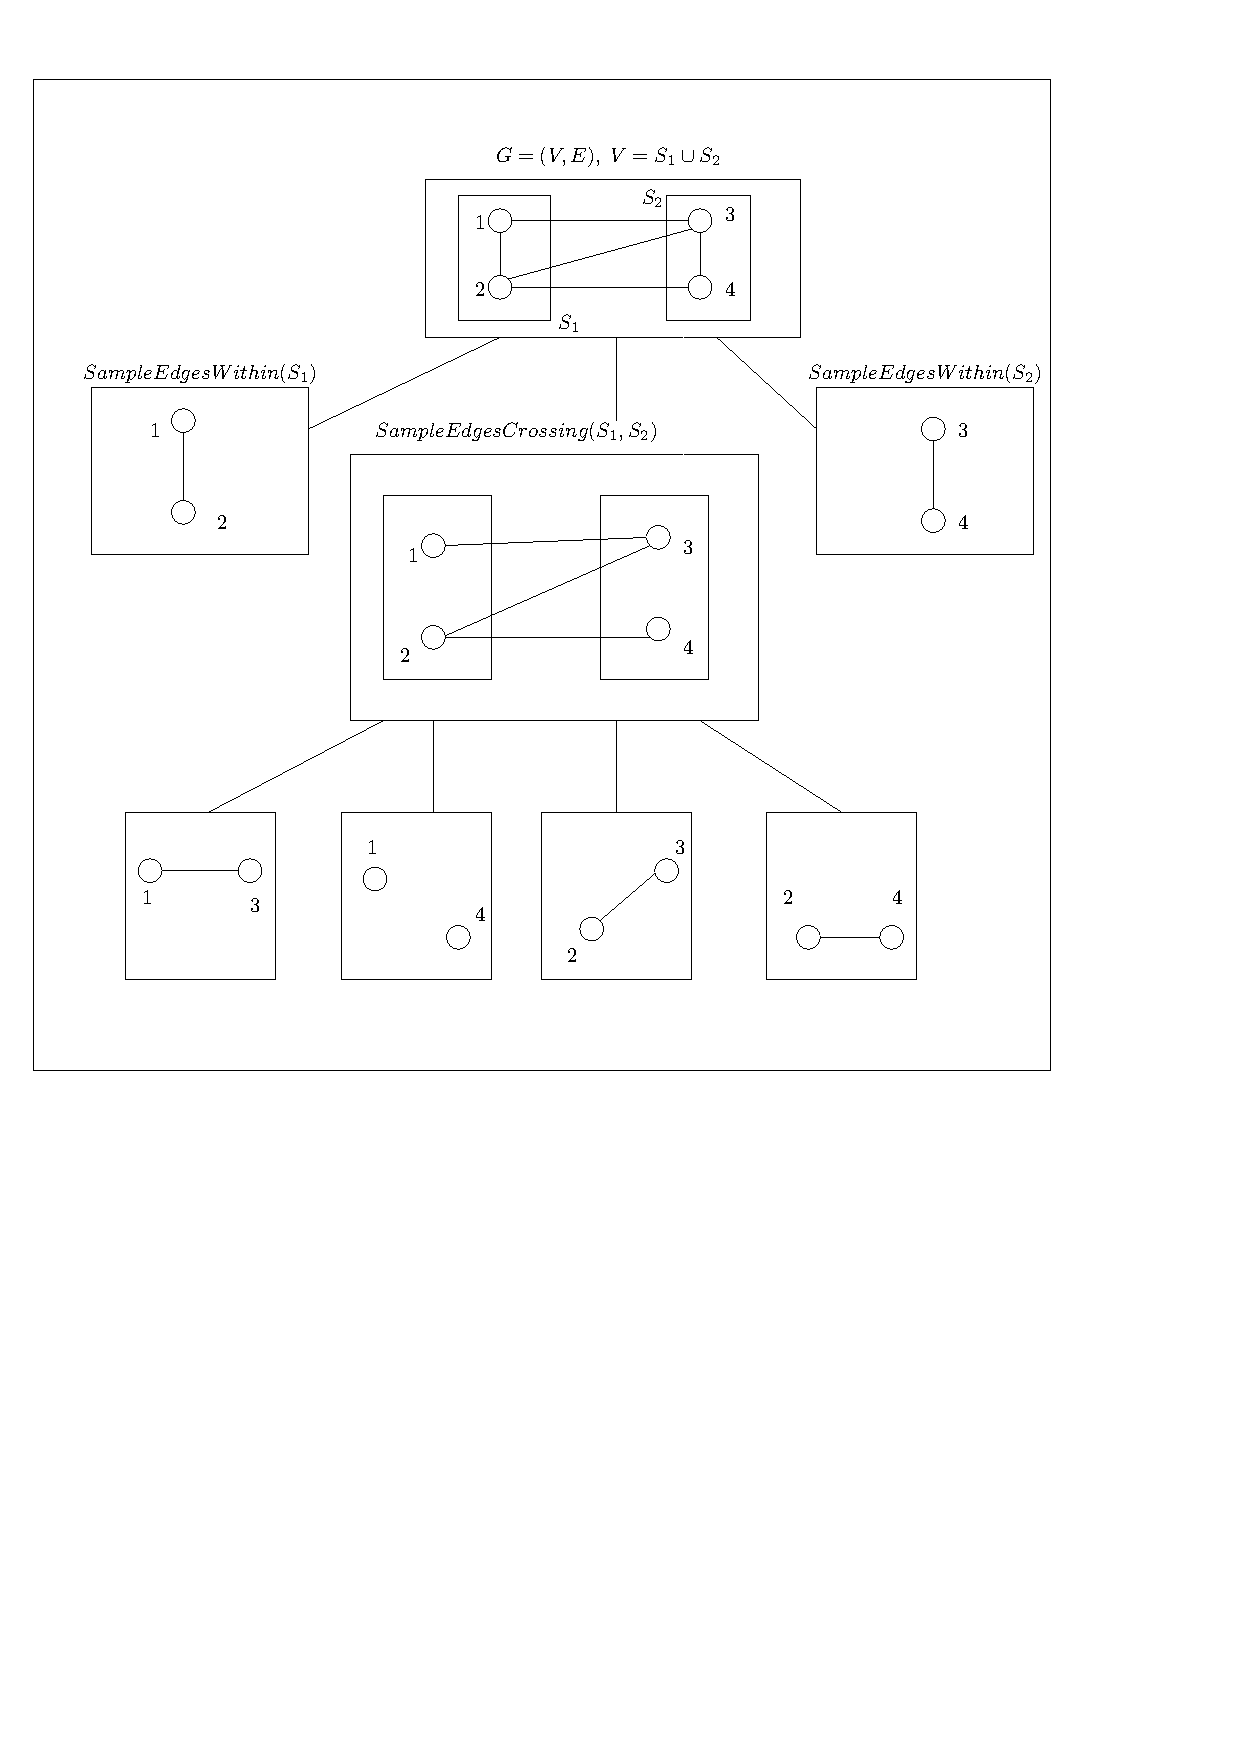
\includegraphics{Figures/alg-tree}
% \end{center}


%----------------------------------------------------------------------------------------






% Chapter 2

\chapter{Laplacian Paradigm} % Main chapter title

\label{Chapter5} % For referencing the chapter elsewhere, use \ref{Chapter2} 

%----------------------------------------------------------------------------------------
\section{Kelner, Madry}

%----------------------------------------------------------------------------------------





 
% Chapter 2

\chapter{Conclusion} % Main chapter title

\label{Chapter6} % For referencing the chapter elsewhere, use \ref{Chapter2} 


We have reviewed some of the algorithms used for sampling a uniform spanning tree. The main impetus for going into the details of \citet{harvey2016generating} is due to the fact that it uses the Sherman-Morrison-Woodbury identity for updating the laplacian pseudoinverse. Recently \citet{DBLP:journals/corr/abs-2004-12739} also used the same identity for showing that \textbf{REACHABILITY} problem is in \texttt{DynFO} + \texttt{Mod} $2(\leq, +, \times)$. Hence we explored the possibility of using the same framework for sampling spanning trees in the dynamic setting. But it turns out that there are a lot of subtleties in coming up with a proper formulation. 

%----------------------------------------------------------------------------------------


%----------------------------------------------------------------------------------------








%----------------------------------------------------------------------------------------
%	THESIS CONTENT - APPENDICES
%----------------------------------------------------------------------------------------

% \appendix % Cue to tell LaTeX that the following "chapters" are Appendices

% Include the appendices of the thesis as separate files from the Appendices folder
% Uncomment the lines as you write the Appendices


% % Appendix A

\chapter{Frequently Asked Questions} % Main appendix title

\label{AppendixA} % For referencing this appendix elsewhere, use \ref{AppendixA}

\section{How do I change the colors of links?}

The color of links can be changed to your liking using:

{\small\verb!\hypersetup{urlcolor=red}!}, or

{\small\verb!\hypersetup{citecolor=green}!}, or

{\small\verb!\hypersetup{allcolor=blue}!}.

\noindent If you want to completely hide the links, you can use:

{\small\verb!\hypersetup{allcolors=.}!}, or even better: 

{\small\verb!\hypersetup{hidelinks}!}.

\noindent If you want to have obvious links in the PDF but not the printed text, use:

{\small\verb!\hypersetup{colorlinks=false}!}.

%\include{Appendices/AppendixB}
%\include{Appendices/AppendixC}

%----------------------------------------------------------------------------------------
%	BIBLIOGRAPHY
%----------------------------------------------------------------------------------------

\printbibliography[heading=bibintoc]

%----------------------------------------------------------------------------------------

\end{document}  
